\documentclass[12pt, a4paper]{ctexart}
\usepackage{geometry}
\geometry{left=2.5cm, right=2.5cm, top=3cm, bottom=3cm}
\usepackage{graphicx}
\usepackage{xcolor}
\usepackage{circuitikz}
\usepackage{subcaption}
\usepackage{float}
\usepackage{amsmath}
\usepackage{listings}
\usetikzlibrary{arrows, shapes.gates.logic.US, positioning}
\ctikzset{
    logic ports=ieee,
    logic ports/scale=0.8,
    multipoles/flipflop/pin spacing=0.4
}
\input{risc-v.tex}
\lstset{
    basicstyle=\ttfamily\small,
    frame=single,
    framesep=5pt,
    xleftmargin=10pt,
    xrightmargin=10pt,
    breaklines=true
}

\begin{document}

% 封面
\begin{titlepage}
    \centering
    \vspace*{5cm}
    {\Huge\bfseries 实验报告\par}
    \vspace{2cm}
    {\Large 课程：数字逻辑与计算机组成\par}
    \vspace{1cm}
    {\Large 实验六：单周期 CPU 设计与测试\par}
    \vspace{4cm}
    {\large 姓名：\underline{\makebox[4cm]{郑袭明}}\par}
    \vspace{1cm}
    {\large 学号：\underline{\makebox[4cm]{251502027}}\par}
    \vspace{1cm}
    {\large 日期：\today\par}
\end{titlepage}

\tableofcontents
\enlargethispage{\baselineskip}
\newpage

\section{实验目的}

\begin{enumerate}
    \item 掌握 RV32I 控制器的设计方法。
    \item 掌握多输入多输出组合逻辑部件设计方法。
    \item 掌握最小风险法设计方法。
    \item 掌握 R32I 单周期 CPU 的设计方法。
    \item 掌握加载程序初始地址和结束程序执行的设计方法。
    \item 掌握计算程序执行周期的设计方法
    \item 理解冯诺依曼程序存储和程序控制的思想
    \item 掌握数据存储器的访问方法
    \item 掌握 RV32I 汇编程序编译方法
    \item 掌握单周期 CPU 加载程序执行的方法
    \item 掌握 RARS 编译仿真工具的使用方法
    \item 掌握冒泡排序算法的设计方法
    \item 数据存储器数据交换的设计方法
    \item 数据存储器数据交换的设计方法
    \item 前后课程实验内容贯通
    \item 掌握代码段和数据段统一编址后的代码文件和数据文件加载方法
    \item 理解 C 语言程序、RISCV 汇编程序与机器语言代码之间的对应关系。
\end{enumerate}

\section{实验一：控制器设计实验}

\subsection{整体方案设计}

使用复杂逻辑门，用 opcode, func3, func7 来输出各控制信号。

以下为引脚功能表

\begin{itemize}
    \item \textbf{ExtOp:} 立即数产生器的控制信号，根据指令类型赋值，宽度为 3 位。
    \item \textbf{ALUASrc:} ALU 输入端 A 的选择信号，0: R[Rs1], 1: PC。
    \item \textbf{ALUBSrc:} ALU 输入端 B 的选择信号，宽度为 2 位，00: R[Rs2], 01: 4, 10: imm。
    \item \textbf{ALUctr:} ALU 控制信号，根据指令操作码和功能码赋值，宽度为 4 位。
    \item \textbf{MemOp:} 数据存储器读写操作以及字节长度控制信号，宽度为 3 位。
    \item \textbf{RegWr:} 寄存器堆写使能控制信号，根据指令类型在相应的执行阶段来赋值，高电平有效。
    \item \textbf{MemWr:} 数据存储器写使能控制信号，高电平有效。
    \item \textbf{BandJ:} 用于分支跳转控制器的输入，生成下地址逻辑部件中控制信号 NPCASrc 和 NPCBSrc，宽度为 3 位。
    \item \textbf{MemtoReg:} 寄存器堆写入数据来源控制信号，0: ALU 运算结果，1: 数据存储器读取输出。
    \item \textbf{NPCASrc:} 下地址逻辑中加法器输入端 A 的选择信号，0: PC, 1: R[Rs1]。
    \item \textbf{NPCBSrc:} 下地址逻辑中加法器输入端 B 的选择信号，0: 4, 1: imm。
\end{itemize}

\subsection{电路设计}

\begin{figure}[H]
    \centering
    \begin{circuitikz}
        \node[
            muxdemux,
            muxdemux def={Lh=4, Rh=4, w=4, NL=3, NR=1, NT=0, NB=0}
        ] (logic) {Gates};
        \node[left] at (logic.lpin 1) {opcode[6:0]};
        \node[left] at (logic.lpin 2) {func3[2:0]};
        \node[left] at (logic.lpin 3) {func7[5]};
        \node[right] at (logic.rpin 1) {Output};
    \end{circuitikz}
    \caption{控制器设计实验原理图}
\end{figure}

\begin{figure}[H]
    \centering
    
\includegraphics[width=0.8\textwidth]{assets/exp1/circuit.png}
    \caption{控制器设计实验电路图}
\end{figure}

\subsection{仿真结果}

\begin{figure}[H]
    \centering
    \subcaptionbox{}{
\includegraphics[width=0.8\textwidth]{assets/exp1/sim1.png}}
    \subcaptionbox{}{
\includegraphics[width=0.8\textwidth]{assets/exp1/sim2.png}}
    \caption{控制器设计实验仿真结果}
\end{figure}

\begin{table}[H]
    \centering
    \small
    \begin{tabular}{cccccccccc}
        \hline
        指令 & 类型 & op[6:0] & func3 & func7[5] & ExtOp & RegWr & ALUASrc & ALUBSrc & ALUctr \\
        \hline
        lui & U & 110111 & X & X & 1 & 1 & X & 10 & 1111 \\
        auipc & U & 010111 & X & X & 1 & 1 & 1 & 10 & 0 \\
        addi & I & 010011 & 0 & X & 0 & 1 & 0 & 10 & 0 \\
        slti & I & 010011 & 10 & X & 0 & 1 & 0 & 10 & 10 \\
        sltiu & I & 010011 & 11 & X & 0 & 1 & 0 & 10 & 11 \\
        xori & I & 010011 & 100 & X & 0 & 1 & 0 & 10 & 100 \\
        ori & I & 010011 & 110 & X & 0 & 1 & 0 & 10 & 110 \\
        andi & I & 010011 & 111 & X & 0 & 1 & 0 & 10 & 111 \\
        slli & I & 010011 & 1 & 0 & 0 & 1 & 0 & 10 & 1 \\
        srli & I & 010011 & 101 & 0 & 0 & 1 & 0 & 10 & 101 \\
        srai & I & 010011 & 101 & 1 & 0 & 1 & 0 & 10 & 1101 \\
        add & R & 0110011 & 0 & 0 & X & 1 & 0 & 0 & 0 \\
        sub & R & 0110011 & 0 & 1 & X & 1 & 0 & 0 & 1000 \\
        sll & R & 0110011 & 1 & 0 & X & 1 & 0 & 0 & 1 \\
        slt & R & 0110011 & 10 & 0 & X & 1 & 0 & 0 & 10 \\
        sltu & R & 0110011 & 11 & 0 & X & 1 & 0 & 0 & 11 \\
        xor & R & 0110011 & 100 & 0 & X & 1 & 0 & 0 & 100 \\
        srl & R & 0110011 & 101 & 0 & X & 1 & 0 & 0 & 101 \\
        sra & R & 0110011 & 101 & 1 & X & 1 & 0 & 0 & 1101 \\
        or & R & 0110011 & 110 & 0 & X & 1 & 0 & 0 & 110 \\
        and & R & 0110011 & 111 & 0 & X & 1 & 0 & 0 & 111 \\
        jal & J & 1101111 & X & X & 100 & 1 & 1 & 1 & 0 \\
        jalr & I & 1100111 & 0 & X & 0 & 1 & 1 & 1 & 0 \\
        beq & B & 1100011 & 0 & X & 11 & 0 & 0 & 0 & 10 \\
        bne & B & 1100011 & 1 & X & 11 & 0 & 0 & 0 & 10 \\
        blt & B & 1100011 & 100 & X & 11 & 0 & 0 & 0 & 10 \\
        bge & B & 1100011 & 101 & X & 11 & 0 & 0 & 0 & 10 \\
        bltu & B & 1100011 & 110 & X & 11 & 0 & 0 & 0 & 11 \\
        bgeu & B & 1100011 & 111 & X & 11 & 0 & 0 & 0 & 11 \\
        lb & I & 0000011 & 0 & X & 0 & 1 & 0 & 10 & 0 \\
        lh & I & 0000011 & 1 & X & 0 & 1 & 0 & 10 & 0 \\
        lw & I & 0000011 & 10 & X & 0 & 1 & 0 & 10 & 0 \\
        lbu & I & 0000011 & 100 & X & 0 & 1 & 0 & 10 & 0 \\
        lhu & I & 0000011 & 101 & X & 0 & 1 & 0 & 10 & 0 \\
        sb & S & 0100011 & 0 & X & 10 & 0 & 0 & 10 & 0 \\
        sh & S & 0100011 & 1 & X & 10 & 0 & 0 & 10 & 0 \\
        sw & S & 0100011 & 10 & X & 10 & 0 & 0 & 10 & 0 \\
        \hline
    \end{tabular}
    \caption{控制器设计实验真值表}
\end{table}

\begin{table}[H]
    \centering
    \small
    \begin{tabular}{cccccccccc}
        \hline
        指令 & 类型 & op[6:0] & func3 & func7[5] & BandJ & MemtoReg & MemWr & MemOp \\
        \hline
        lui & U & 110111 & X & X & 0 & 0 & 0 & X \\
        auipc & U & 010111 & X & X & 0 & 0 & 0 & X \\
        addi & I & 010011 & 0 & X & 0 & 0 & 0 & X \\
        slti & I & 010011 & 10 & X & 0 & 0 & 0 & X \\
        sltiu & I & 010011 & 11 & X & 0 & 0 & 0 & X \\
        xori & I & 010011 & 100 & X & 0 & 0 & 0 & X \\
        ori & I & 010011 & 110 & X & 0 & 0 & 0 & X \\
        andi & I & 010011 & 111 & X & 0 & 0 & 0 & X \\
        slli & I & 010011 & 1 & 0 & 0 & 0 & 0 & X \\
        srli & I & 010011 & 101 & 0 & 0 & 0 & 0 & X \\
        srai & I & 010011 & 101 & 1 & 0 & 0 & 0 & X \\
        add & R & 0110011 & 0 & 0 & 0 & 0 & 0 & X \\
        sub & R & 0110011 & 0 & 1 & 0 & 0 & 0 & X \\
        sll & R & 0110011 & 1 & 0 & 0 & 0 & 0 & X \\
        slt & R & 0110011 & 10 & 0 & 0 & 0 & 0 & X \\
        sltu & R & 0110011 & 11 & 0 & 0 & 0 & 0 & X \\
        xor & R & 0110011 & 100 & 0 & 0 & 0 & 0 & X \\
        srl & R & 0110011 & 101 & 0 & 0 & 0 & 0 & X \\
        sra & R & 0110011 & 101 & 1 & 0 & 0 & 0 & X \\
        or & R & 0110011 & 110 & 0 & 0 & 0 & 0 & X \\
        and & R & 0110011 & 111 & 0 & 0 & 0 & 0 & X \\
        jal & J & 1101111 & X & X & 1 & 0 & 0 & X \\
        jalr & I & 1100111 & 0 & X & 10 & 0 & 0 & X \\
        beq & B & 1100011 & 0 & X & 100 & X & 0 & X \\
        bne & B & 1100011 & 1 & X & 101 & X & 0 & X \\
        blt & B & 1100011 & 100 & X & 110 & X & 0 & X \\
        bge & B & 1100011 & 101 & X & 111 & X & 0 & X \\
        bltu & B & 1100011 & 110 & X & 110 & X & 0 & X \\
        bgeu & B & 1100011 & 111 & X & 111 & X & 0 & X \\
        lb & I & 0000011 & 0 & X & 0 & 1 & 0 & 101 \\
        lh & I & 0000011 & 1 & X & 0 & 1 & 0 & 110 \\
        lw & I & 0000011 & 10 & X & 0 & 1 & 0 & 0 \\
        lbu & I & 0000011 & 100 & X & 0 & 1 & 0 & 1 \\
        lhu & I & 0000011 & 101 & X & 0 & 1 & 0 & 10 \\
        sb & S & 0100011 & 0 & X & 0 & X & 1 & 101 \\
        sh & S & 0100011 & 1 & X & 0 & X & 1 & 110 \\
        sw & S & 0100011 & 10 & X & 0 & X & 1 & 0 \\
        \hline
    \end{tabular}
    \caption{控制器设计实验真值表}
\end{table}

\subsection{错误现象及分析}

在完成实验的过程中，没有遇到任何错误。

\section{实验二：单周期CPU设计实验}

\subsection{整体方案设计}

\begin{figure}[H]
    \centering
    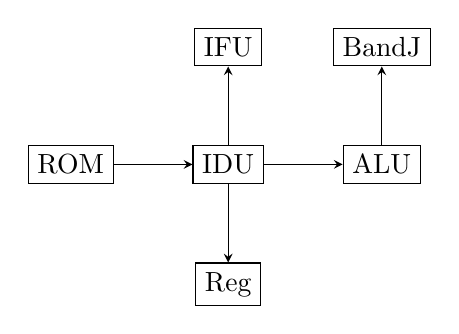
\begin{tikzpicture}[>=stealth]
        \node[draw] (idu) {IDU};
        \node[draw, below=of idu] (reg) {Reg};
        \node[draw, right=of idu] (alu) {ALU};
        \node[draw, above=of alu] (bandj) {BandJ};
        \node[draw, left=of idu] (rom) {ROM};
        \node[draw, above=of idu] (ifu) {IFU};
        \draw[->] (rom) -- (idu);
        \draw[->] (idu) -- (reg);
        \draw[->] (idu) -- (ifu);
        \draw[->] (idu) -- (alu);
        \draw[->] (alu) -- (bandj);
    \end{tikzpicture}
    \caption{单周期CPU设计实验整体方案设计}
\end{figure}

\subsection{电路设计}

\begin{figure}[H]
    \centering
    
\includegraphics[width=0.8\textwidth]{assets/exp2/sch.png}
    \caption{单周期CPU设计实验原理图}
\end{figure}

\begin{figure}[H]
    \centering
    
\includegraphics[width=0.8\textwidth]{assets/exp2/circuit.png}
    \caption{单周期CPU设计实验电路图}
\end{figure}

\subsection{仿真结果}

\begin{figure}[H]
    \centering
    
\includegraphics[width=0.8\textwidth]{assets/exp2/circuit.png}
    \caption{单周期CPU设计实验电路图}
\end{figure}

\subsection{仿真结果}

\begin{figure}[H]
    \centering
    \subcaptionbox{}{
\includegraphics[width=0.8\textwidth]{assets/exp2/sim1.png}}
    \subcaptionbox{}{
\includegraphics[width=0.8\textwidth]{assets/exp2/sim2.png}}
    \caption{单周期CPU设计实验仿真结果}
\end{figure}

\subsection{错误现象及分析}

在完成实验的过程中，没有遇到任何错误。

\section{实验三：累加和程序测试实验}

\subsection{整体方案设计}

\begin{lstlisting}[language={[RISC-V]Assembler}]
main:
    lbu     a1, 0(x0)
    beq     a1, x0, fail
    ori     a2, x0, 1
    xor     a3, a3, a3
loop:
    add     a3, a3, a2
    beq     a2, a1, finish
    addi    a2, a2, 1
    jal     x0, loop 
finish:
    sw a3, 4(x0)
pass:
    lui	    a0,0xc10
    addi	a0,a0,-18
    ecall
fail:
    lui	    a0, 0xdeade
    addi	a0, a0, -339
    ecall
\end{lstlisting}

\subsection{电路设计}

见单周期CPU设计实验电路图。

\subsection{仿真结果}

\begin{figure}[H]
    \centering
    \subcaptionbox{}{
\includegraphics[width=0.8\textwidth]{assets/exp3/sim1.png}}
    \subcaptionbox{}{
\includegraphics[width=0.8\textwidth]{assets/exp3/sim2.png}}
    \caption{累加和程序测试实验仿真结果}
\end{figure}

\subsection{错误现象及分析}

在完成实验的过程中，没有遇到任何错误。

\section{实验四：冒泡排序程序测试实验}

\subsection{整体方案设计}

\begin{lstlisting}[language={[RISC-V]Assembler}]
main:
	lw      t0, 0(x0)
	addi    a1, x0, 1
	add     a2, t0, x0
L1:
	addi    a3, x0, 1
L2:
    slli    a4, a3, 2
	lw      a6, 0(a4)
	lw      a7, 4(a4)
	bge     a7, a6, L4
	sw      a7, 0(a4)
	sw      a6, 4(a4)
L4:	
	addi    a3, a3, 1
	bltu    a3, a2, L2
L3:
    sub     a2, a2, a1
    bne     a2, a1, L1
    ecall
\end{lstlisting}

\subsection{电路设计}

见单周期CPU设计实验电路图。

\subsection{仿真结果}

\begin{figure}[H]
    \centering
    \subcaptionbox{}{
\includegraphics[width=0.8\textwidth]{assets/exp4/sim1.png}}
    \subcaptionbox{}{
\includegraphics[width=0.8\textwidth]{assets/exp4/sim2.png}}
    \caption{冒泡排序程序测试实验仿真结果}
\end{figure}

\subsection{错误现象及分析}

在完成实验的过程中，没有遇到任何错误。

\section{实验五：官方测试集实验}

\begin{table}[H]
    \centering
    \small
    \begin{tabular}{cccccc}
        \hline
        序号 & 测试指令 & x1寄存器输出值 & x3寄存器输出值 & x10寄存器输出值 & 时钟周期数 \\
        \hline
        1 & add & 0x00000010 & 0x00000026 & 0xc0ffee & 457 \\
        2 & addi & 0x00000021 & 0x00000019 & 0xc0ffee & 234 \\
        3 & and & 0x11111111 & 0x0000001b & 0xc0ffee & 477 \\
        4 & andi & 0x00ff00ff & 0x0000000e & 0xc0ffee & 190 \\
        5 & auipc & 0x00000000 & 0x00000003 & 0xc0ffee & 51 \\
        6 & beq & 0x00000003 & 0x00000015 & 0xc0ffee & 283 \\
        7 & bge & 0x00000003 & 0x00000018 & 0xc0ffee & 301 \\
        8 & bgeu & 0x00000003 & 0x00000018 & 0xc0ffee & 326 \\
        9 & blt & 0x00000003 & 0x00000015 & 0xc0ffee & 283 \\
        10 & bltu & 0x00000003 & 0x00000015 & 0xc0ffee & 308 \\
        11 & bne & 0x00000003 & 0x00000015 & 0xc0ffee & 283 \\
        12 & jal & 0x00000003 & 0x00000003 & 0xc0ffee & 47 \\
        13 & jalr & 0x00000000 & 0x00000007 & 0xc0ffee & 107 \\
        14 & lb & 0x00002000 & 0x00000013 & 0xc0ffee & 237 \\
        15 & lbu & 0x00002000 & 0x00000013 & 0xc0ffee & 237 \\
        16 & lh & 0x00002000 & 0x00000013 & 0xc0ffee & 249 \\
        17 & lhu & 0x00002000 & 0x00000013 & 0xc0ffee & 256 \\
        18 & lui & 0xfffff800 & 0x00000006 & 0xc0ffee & 57 \\
        19 & lw & 0x00002000 & 0x00000013 & 0xc0ffee & 259 \\
        20 & or & 0x11111111 & 0x0000001b & 0xc0ffee & 480 \\
        21 & ori & 0x00ff00ff & 0x0000000e & 0xc0ffee & 197 \\
        22 & sb & 0x00000001 & 0x00000017 & 0xc0ffee & 422 \\
        23 & sh & 0x00003001 & 0x00000017 & 0xc0ffee & 475 \\
        24 & sll & 0x00000400 & 0x0000002b & 0xc0ffee & 485 \\
        25 & slli & 0x00000021 & 0x00000019 & 0xc0ffee & 233 \\
        26 & slt & 0x00000010 & 0x00000026 & 0xc0ffee & 451 \\
        27 & slti & 0x00ff00ff & 0x00000019 & 0xc0ffee & 229 \\
        28 & sltiu & 0x00ff00ff & 0x00000019 & 0xc0ffee & 229 \\
        29 & sltu & 0x00000010 & 0x00000026 & 0xc0ffee & 451 \\
        30 & sra & 0x00000400 & 0x0000002b & 0xc0ffee & 504 \\
        31 & srai & 0x00000021 & 0x00000019 & 0xc0ffee & 248 \\
        32 & srl & 0x00000400 & 0x0000002b & 0xc0ffee & 498 \\
        33 & srli & 0x00000021 & 0x00000019 & 0xc0ffee & 242 \\
        34 & sub & 0x00000010 & 0x00000025 & 0xc0ffee & 449 \\
        35 & sw & 0x12233001 & 0x00000017 & 0xc0ffee & 482 \\
        36 & xor & 0x11111111 & 0x0000001b & 0xc0ffee & 479 \\
        37 & xori & 0x00ff00ff & 0x0000000e & 0xc0ffee & 199 \\
        \hline
    \end{tabular}
\end{table}

\begin{enumerate}
    \item \textbf{fib1.asm} \quad 指令存储器加载：fib1.hex \\
    数据存储器0x2000依次加载：0x0a, 0x1e, 0x28, 0x3c \\
    执行周期数：70 \quad 190 \quad 250 \quad 370 \\
    执行结果，数据存储器地址 M[0x2004] 中的结果： \\
    0x00000037, 0x000cb228, 0x06197ecb, 0x6c8312d0 \\
    如何优化程序？

    \item \textbf{mul1.asm} \quad 指令存储器加载：mul1.hex， \\
    数据存储器0x2000、0x2004分别依次加载：0x000000ff, 0x00000064; 0x0000ffff, 0x0000ffff \\
    执行周期数：54 \quad 121 \\
    执行结果，寄存器堆x7： \\
    0x0000639c, 0xfffe0001

    \item \textbf{divl1.asm} \quad 指令存储器加载：div1.hex， \\
    数据存储器0x2000、0x2004分别依次加载：0x0000fff0, 0x00000e7; 0x00ffff00, 0x000000fe \\
    执行周期数：1141 \quad 1041 \\
    执行结果，寄存器堆x7：x5： \\
    0x0000011b, 0x00000093, 0x00000102, 0x00000300

    \item \textbf{array-add.asm} \quad 指令存储器加载：array-add.hex， \\
    数据存储器ram0加载 array-add.dat \\
    执行周期数：87 \\
    执行结果：读取数据存储器0x200开始的10个数据： \\
    0xffffff58, 0x0000004c, 0xffffffba, 0x000000ac, 0xffffffea, 0x00000086, 0x0000000b, 0x000000a5, 0x00000059, 0xffffffa2
\end{enumerate}

\section{实验六：计算机系统基础 PA 程序测试实验}

\subsection{b-sort 程序测试}

指令存储器加载：b-sort-riscv32-npc.bin-logisim-inst.txt

数据存储器分别加载：b-sort-riscv32-npc.bin-logisim-data0-3.txt

程序执行周期数：1348

\begin{figure}[H]
    \centering
    \subcaptionbox{开始时}{
\includegraphics[width=0.8\textwidth]{assets/exp6/sim1.png}}
    \subcaptionbox{结束时}{
\includegraphics[width=0.8\textwidth]{assets/exp6/sim2.png}}
    \caption{b-sort 程序测试实验仿真结果}
\end{figure}

\section{思考题}

\subsection{在单 CPU 上实现多任务处理}

采用时间片轮转的多任务调度机制。通过定时器产生硬件中断，操作系统在中断服务程序中保存当前任务的上下文，调用调度算法选择下一任务，恢复其上下文并跳转执行，实现宏观上的并发。

\subsection{在 CPU 的基础上实现输入输出设备的数据访问}

建立系统总线，采用统一编址或独立编址，为键盘和TTY分配地址。采用轮询或中断机制进行数据交互：CPU通过读取键盘接口寄存器获取输入，向TTY接口寄存器写入数据实现输出，从而构成系统。

\subsection{在单周期 CPU 基础上实现多周期 CPU}

将单周期指令执行过程拆分为取指、译码、执行、访存、写回等多周期。在各阶段间引入暂存器（如IR、MDR）保存中间结果，并设计有限状态机控制器，根据当前状态和指令分步输出控制信号，实现资源复用。

\subsection{单周期 CPU 基础上实现流水线 CPU}

在单周期各功能部件间插入流水线寄存器，将指令执行划分为多个并行阶段。每个时钟周期各阶段同时处理不同指令。需设计冲突检测逻辑，采用旁路前推、插入气泡或分支预测来解决数据和控制冲突。

\end{document}
